%%%%%%%%%%%%%%%%%%%%%%%%%%%%%%%%%%%%%%%%%%%%%%%%%%%%%%%%%%%%%%%%%%%%%%%%%%%%%%%%
%2345678901234567890123456789012345678901234567890123456789012345678901234567890
%        1         2         3         4         5         6         7         8

\documentclass[letterpaper, 10 pt, conference]{ieeeconf}  % Comment this line out
                                                          % if you need a4paper
%\documentclass[a4paper, 10pt, conference]{ieeeconf}      % Use this line for a4
                                                          % paper

\IEEEoverridecommandlockouts                              % This command is only
                                                          % needed if you want to
                                                          % use the \thanks command
\overrideIEEEmargins
% See the \addtolength command later in the file to balance the column lengths
% on the last page of the document

\usepackage{graphicx}
\usepackage{multirow}
\usepackage{url}
\usepackage[utf8]{inputenc}
\usepackage{tabularx,booktabs}
\usepackage{pgfplots}
\graphicspath{ {images/} }


% The following packages can be found on http:\\www.ctan.org
%\usepackage{graphics} % for pdf, bitmapped graphics files
%\usepackage{epsfig} % for postscript graphics files
%\usepackage{mathptmx} % assumes new font selection scheme installed
%\usepackage{times} % assumes new font selection scheme installed
%\usepackage{amsmath} % assumes amsmath package installed
%\usepackage{amssymb}  % assumes amsmath package installed

\title{\LARGE \bf
Towards Unsupervised Learning in Medical Image Segmentation: A Survey
}

\author{Marc Moreno Lopez$^{1}$ and William D. Michael$^{2}$% <-this % stops a space
\thanks{*This work is submitted for CS 6000 at the University of Colorado Colorado Springs}% <-this % stops a space
\thanks{$^{1}$M. Moreno Lopez is a student of Computer Science at the University of Colorado - Colorado Springs
        {\tt\small mmorenol@uccs.edu}}%
\thanks{$^{2}$W. D. Michael is a student of Computer Science at the University of Colorado - Colorado Springs
        {\tt\small bmichael@uccs.edu}}%
}

\begin{document}

\maketitle
\thispagestyle{empty}
\pagestyle{empty}

%%%%%%%%%%%%%%%%%%%%%%%%%%%%%%%%%%%%%%%%%%%%%%%%%%%%%%%%%%%%%%%%%%%%%%%%%%%%%%%%
\begin{abstract}

The lack of large annotated datasets is a problem in many fields, specially in medical related fields. Many unsupervised algorithms have been developed in renowned areas of Computer Vision like biometrics and depth estimation. However, these unsupervised techniques hven't been widely applied yet to medical segmentation. In this paper we will review the most well-known supervised techniques for medical segmentation and we will review novel techniques for unsupervised learning.

\end{abstract}

%%%%%%%%%%%%%%%%%%%%%%%%%%%%%%%%%%%%%%%%%%%%%%%%%%%%%%%%%%%%%%%%%%%%%%%%%%%%%%%%
\section{INTRODUCTION}
In this paper, we will examine segmentation of medical imagery. Segmentation of these images is a critical step for applying machine learning to image analysis and understanding. but supervised segmentation techniques - ubiquitous in other applications -  lacks the with an emphasis on unsupervised segmentation. 

In an older survey of the use of machine learning for medical imagery, Pham et al captured the essence of segmentation: "Image segmentation plays a crucial role in many medical-imaging applications, by automating or facilitating the delineation of anatomical structures and other regions of interest" \cite{pham2000current}.

Although unsupervised segmentation is generally desirable, in many areas of computer vision, supervised segmentation approaches exhibit better performance as a result of extensive training using large, manually segmented datasets. We will briefly survey supervised and semi-supervised learning but the major emphasis will be \textit{unsupervised learning}. Segmentation using supervised learning has been extensively researched with performance correlating closely with the size of the dataset used for training. Large annotated datasets exist for many problems such as autonomous driving, image classification and activity recognition because images can be inexpensively annotated by relatively low-skilled analysts. Large datasets do not, however, exist for many important problems, notably those involving segmentation of medical data. Few such datasets exist for medical imagery, primarily for the following reasons (this probably isn't the best place to use a bullet list but I wanted to try it in \LaTeX{}):

\begin{itemize}
    \item Most medical images are not visual but are created using x-ray or magnetic resonance imaging (MRI). Annotation of imagery created with these technologies requires extensive training. Consequently, such datasets are expensive to create.  As a result there is a startling lack of such imagery compared to other areas of research, such as autonomous driving.
    \item Further contributing to the scarcity of freely available data, the consent of the patient, medical organization and medical provider are required before imagery can be included in a dataset.
\end{itemize}
 
While we would like to limit our analysis to medical imagery, the vast majority of segmentation research has been conducted with non-medical imagery. Accordingly, we have attempted to juxtapose other relevant segmentation research with medical image segmentation. Exacerbating the lack of annotated medical imagery is the soft tissue deformation results in different presentation of anatomical structure among different subjects. We found little research contemporary research using deep learning for segmenting deformable objects found in medical imagery although it was previously an are of interest \cite{mcinerney1996deformable} \cite{yangdeformable20043d}. Deep learning might be expected to accommodate segmentation in the presence of deformation but the dearth of training datasets portraying deformation resulting from pathology leads to the conclusion that DLN may not perform well when the images present more deformation than is present in the training data. We found only one paper that combined ML with a deformable model \cite{avendi_combined_2016}. 

With this paper we intend to introduce and review some of the most successful learning methods that have been used in prominent areas of Computer Vision ultimately emphasizing unsupervised learning. Supervised methods have achieved excellent results but will remain impractical for many applications including medical imaging. For these applications, unsupervised segmentation or supervised learning using very small training datasets) remains an imperative. Until such methods are available, the large scale exploitation of medical imagery for machine learning will remain an unachievable goal. Further contibuting to the lack of training data is the difficulty of augmenting medical imagery. Traditional data techniques such as mirroring, translating and cropping are frequently inappropriate due to the nature of imaging techniques employed.

A previous approach to a survey on unsupervised learning methods was done in 2012 by Bengio et al \cite{bengio_representation_2012}. They reviewed work in the area of unsupervised feature learning and deep learning, including probabilistic models, manifold learning, and deep learning. This motivates longer-term unanswered questions about the appropriate objectives for learning good representations, for computing representations (i.e., inference), and the geometrical connections between representation learning, density estimation and manifold learning.

As DNN approaches dominate research in segmentation of medical imagery, we note that in 1998 Vilarino et al \cite{vilarino_discrete-time_1998} presaged the future of this research by proposing a "multi-layer cellular neural network"  approach to biomedical image segmentation. Vilarino's segmentation strategy detected active contours by implementing a multilayer cellular neural network contour detector. The approach consisted of an "expanding and thinning process, guided by external information" from a contour which evolves until it reaches the final desired position in the image processed. Although the approach is somewhat limited by today's standards, we observe that this effort remains relevant nearly two decades later.

\section{SUPERVISED LEARNING FOR SEGMENTATION}
% \begin{figure}
%  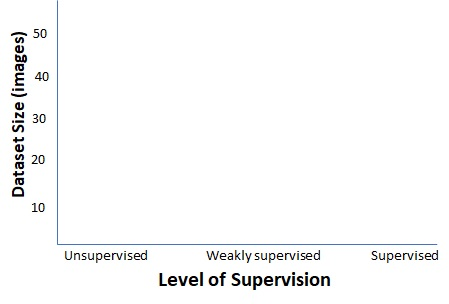
\includegraphics[width=\linewidth]{images/SupervisionvsDatasetSize.jpg}
%  \caption{Comparison of level of supervision and dataset size}
%   \label{fig:supervdata}
% \end{figure}

Supervised learning for segmentation has been employed with favorable results adequate training data exists. Current supervised segmentation research uses large annotated datasets featuring thousands of unique objects, hundreds of thousands of annotated images and millions of video frames \cite{xu2018youtube}. As mentioned above, the availability of such datasets is unusual in medical segmentation. Before discussing supervised segmentation used for medical imagery, we will discuss the state-of-the-art supervised segmentation efforts. Current segmentation systems those based on AlexNet \cite{krizhevsky_imagenet_2012}, VGG \cite{simonyan_very_deep}, GoogleNet \cite{szegedy_deeper}, ResNet \cite{he_deep_residual} and ReSeg \cite{Visin_2016_CVPR_Workshops}. With the exception of ReSeg, these networks were originally designed as classification networks. To adapt these networks for segmentation, Long et al proposed a modification that replaced the fully connected output and softmax layers with fully convolutional layers \cite{long_fully_2015}. With this modification, the softmax probability vector output was replaced with a spatial map representing a segmentation of the input image. Figure \ref{fig:??} describes each of these networks. Currently, the best segmentation performance is exhibited by systems using fully convolutional neural network (FCNN) implementations.

\begin{figure}
\begin{tikzpicture}
  \begin{axis}
    [   xlabel=Modality,
		ylabel=Tissue Type,
		zlabel=Dataset Size (images)]
     \addplot3[scatter, mark=*,only marks,
           % we use ’point meta’ as color data...
           point meta=\thisrow{color},
           % ... therefore, we can’t use it as argument for nodes near coords
           nodes near coords*={\myvalue},
           % ... which requires to define a visualization dependency:
           visualization depends on={value \thisrow{myvalue} \as \myvalue},
           ]
           table [x=x, y=y, z=z]
           {supervised.txt};
  \end{axis}
\end{tikzpicture}
\caption{Comparison of dataset (using dummy data as I am still figuring out how to present this data)}
\end{figure}

AlexNet was one of the first deep networks to address the classification problem, doing so with a relatively simple architecture that consists of a five convolutional and three fully-connected layers. Originally designed for classification, AlexNet was modified for segmentation by replacing the fully connected final layers with a fully convolutional layers. With this modification, the networks did not output a softmax classification vector but instead output a spatial map with a proposed segmentation of the input image \cite{garcia_article} \cite{krizhevsky_imagenet_2012}. The architecture of the AlexNet classifier is depicted in \ref{fig:alexnet}.

\begin{figure}
  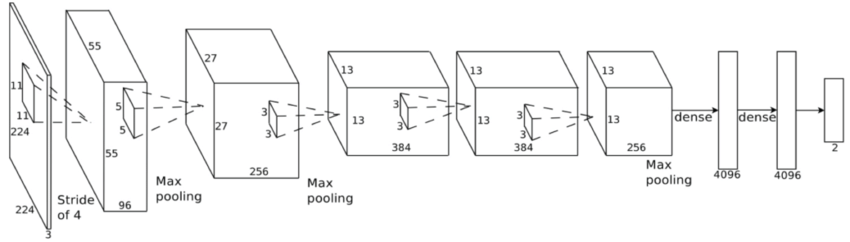
\includegraphics[width=\linewidth]{images/alexnet1.png}
  \caption{Depiction of the AlexNet classifier}
   \label{fig:alexnet}
\end{figure}

Building on AlexNet, the VGG network family investigated the effect of network depth on classification performance \cite{simonyan_VGG}. This network used only 3x3 convolutional filters and 2x2 max pooling layers. The convolution stride is 1 while the pooling convolution stride is 2. As a result of these design constraints, networks can be very deep while avoiding vanishing or exploding gradients. The initial research investigated networks with 11 to 19 weighted layers (as detailed in Figure \ref{fig:VGG}), five weighted layers, three fully connected layers and a softmax output layer. To modify the VGG from the classification task to the segmentation task, fully convolutional layers were placed in the output of the network. 

\begin{figure}
  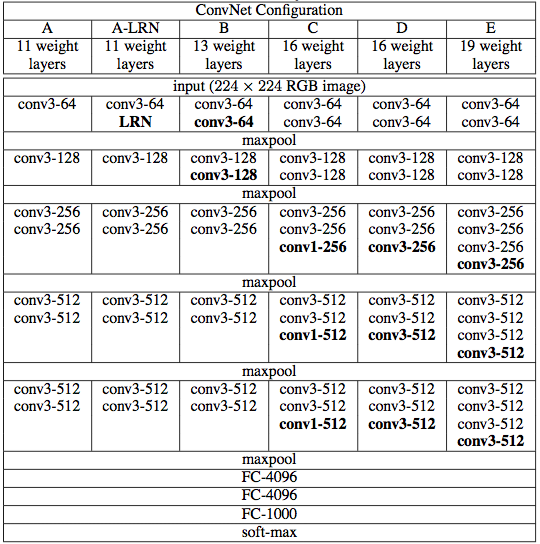
\includegraphics[width=\linewidth]{images/VGG.png}
  \caption{Description of the VGG DNN Network Investigation}
   \label{fig:VGG}
\end{figure}

Inspired by VGG, SegNet modifies the VGG architecture to produce a pixel-by-pixel level segmentation of an image. SegNet extends the idea of using a deconvolutional backend for image segmentation by implementing a convolutional encoder network to determine salient features from an image and then using a decoder to upsample to an image sized segmentation of the input image \cite{badrinarayanan_segnet:_2015}. A depiction of the SegNet architecture is shown in Figure \ref{fig:segnet}.

\begin{figure}
  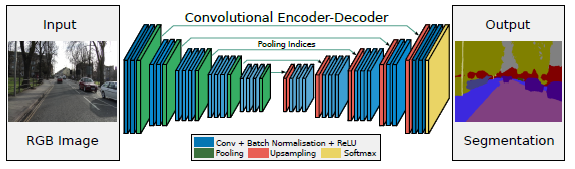
\includegraphics[width=\linewidth]{images/segnet.png}
  \caption{The SegNet Architecture \cite{badrinarayanan_segnet:_2015}}
   \label{fig:segnet}
\end{figure}


Dai et al describe a system that uses an unsupervised discriminant shape (UDS) is used to address category-specific object segmentation by using the proposed shape prior into an intuitive energy minimization framework. Deep CNNs are used to identify candidate segments classified by categories of interest. However, the proposed segments obtained from the CNN tend to undershoot or overshoot objects and are easily classified into one specific class. To address this problem, an unsupervised discriminant projection based clustering algorithm (UDC) to refine a more precises shape prior to segmentation. The class-specific proposals are clustered based on their projections onto the discriminant projection direction. Based on the set of proposals, a voting scheme is used to form the solution. The derived UDS prior is finally utilized in the subsequent energy minimizing formulation based figure-ground segmentation \cite{dai_r-fcn:_2016}. 

Liu et al \cite{liu_semantic_2015} extend the VGG network by incorporating Markov Random Fields (MRF) and Conditional Random Fields (CRF) to create a graph-based segmentation of medical. This network, termed the \textit{Deep Parsing Network} (DPN) segments an image with a single forward pass.  The DPN models patches in the image using four output layers inspired by the mean field algorithm.  

In \cite{badrinarayanan_segnet:_2015}  a trainable segmentation engine (SegNet) consists of an encoder network, a corresponding decoder network followed by a pixel-wise classification layer. Architecture of the encoder network is topologically identical to the 13 convolutional layers in the VGG16 network. The decoder network is to map the low resolution encoder feature maps to full input resolution feature maps for pixel-wise classification. SegNet decoder upsamples its lower resolution input feature map(s); the decoder uses pooling indices computed in the max-pooling step of the corresponding encoder to perform non-linear upsampling. This eliminates the need for learning to upsample [?]. The upsampled maps are sparse and then convolved with trainable filters to produce dense feature maps. SegNet primarily motivated by scene understanding applications and is efficient both in terms of memory and computational time during inference. Also significantly smaller in the number of trainable parameters than other competing architectures. Trained end-to-end using stochastic gradient descent. (SUN RGB-D indoor scene segmentation tasks). Quantitative assessments show competitive inference time and efficient inference memory-wise, compared to other architectures. (Caffe implementation of SegNet and a web demo).

In \cite{dai_r-fcn:_2016}, a region-based, FCNN is used for object detection. In contrast to previous region-based detectors such as Fast/Faster RCNN that apply a costly per-region subnetwork hundreds of times, our region-based detector is fully convolutional with almost all computation shared on the entire image. To achieve this goal, we propose position-sensitive score maps to address a dilemma between translation-invariance in image classification and translation-variance in object detection. Achieved at a test-time speed of 170ms. (PASCAL VOC) Code: https://github.com/daijifeng001/r-fcn.

In \cite{aytekin_learning_graph} graph affinities for salient object detection. A graph representation of an image is created then the net learns to predict affinities related to this graph and analyzed. Uses modified convolutional kernel networks (CKNs) to calculate graph affinity  and estimate similarities between images. Then uses a spectral graph based salient object detection method (Extended Quantum Cuts (EQCut)). Salient object detection error of such a system is differentiable with respect to the parameters of the CKN. This is used for training using backpropagation.  Computationally efficient.

/subsection{Supervised Learning for Segmentation of Medical Imagery}

In light of research described above, we now examine supervised segmentation efforts for medical imagery. A brief synopsis is available in \ref{medical_supervised}. 

\begin{table*}
 \caption{Medical Image Segmentation - Supervised Learning}
\label{medical_supervised}
%\begin{tabularx}{\textwidth}{@{}l*{6}{C}c@{}}
\begin{tabularx}{\textwidth}{@{}l*{6}{c}c@{}}
\toprule
Author & Technology & Anatomy & Training Dataset & Training Dataset Size & Code Available & Reference \\  
\midrule
 Miletari et al & MR & Prostate & Promise2012 & 50 & Yes & \cite{milletari_vnet} \\ [1ex] 
 \hline
Gibson et al & Generic 2D and 3D & Multiple & Not specified & Unknown & Yes & \cite{gibson_niftynet:_2018} \\ 
 \hline
 Avendi et al & MR & Cardiac LV & MICCAI2009 & 45 & No & \cite{avendi_combined_2016} \\
 \hline
 Zhao et al & MR & Cardiac LV & BRATS2013-2016 & 53-110 & No & \cite{zhao_deep_2018} \\
 \hline
 Moeskops et al & MR & Brain & NeoBrainS12/MRBrainS13 & 5-20 & No & \cite{Moeskops_automatic_segmentation} \\
 \hline
 Ngo et al & MR-cine & Cardiac LV & MICCAI 2009 & 15 & No & \cite{NgoLC17_combining} \\ [1ex] 
 \hline
Liskowski et al & Photographic image & Eye & DRIVE & 40 & No & \cite{liskowski_segmenting_2016} \\ [1ex] 
& Photographic image & Eye & STARE & 20 &  &  \\ [1ex] 
& Photographic image & Eye & CHASE & 28 &  &  \\ [1ex] 
 \hline
 Kamnitsas et al & MR & Brain & BRATS2015 & 46 & Yes & \cite{kamnitsas_unsupervised_2017} \\  
 & MR & Brain & ISLES 2015 & 28   \\  
 \hline
 Prasoon et al & MR & Knee & Not specified & 25 & No & \cite{prasoon_deep_2013} \\  
 \hline
 Zhang et al & MR & Brain & Not specified & 10 & No & \cite{zhang_deep_2015} \\ [1ex] 
 \hline
\bottomrule
\end{tabularx}
\end{table*}

Data for medical imagery is frequently much different than data encountered in other computer vision and machine learning tasks. For instance, data may be 2 dimensional (eg, x-ray or fundus imagery), 3-dimensional (MRI) or even higher dimension (eg, MR-cine) \cite{gibson_niftynet:_2018}. Further, the data sought from such imagery also differs from typcial CV and ML tasks. For example, the ejection fraction of the cardiac left ventricle \cite{avendi_combined_2016}\cite{chen_deeplab:_2018}\cite{NgoLC17_combining} is of significant diagnostic interest when analyzing MR-cine imagery. The diversity of imagery and data sought from the imagery result in a wide variety of approaches to applying ML to the medical segmentation task.

Miletari et al \cite{milletari_vnet} describe \textit{V-Net} an approach to 3D image segmentation based on volumetric FCNNs specifically designed for medical image segmentation. Inspired by VGG and other fully convolutional neural networks, the V-Net architecture, depicted in \ref{fig:miletari}, has been used as the basis for several other medical segmentation systems [need cites here]. In this paper, V-Netis trained end-to-end on prostate MRI volumes, with the goal of learning to predict segmentation for the 3D MRI-based volume of the prostate. The loss function directly uses the Dice coefficient to optimize segmentation during training instead of other indirect metrics used by other ML approaches. In the prostate trials described in this paper, V-Net segmented prostate images even in the presence of strong imbalances between the number of foreground and background voxels with Dice scores of [xx]. Due to the limited number of annotated volumes available for training, data is augmented by applying random non-linear transformations to the available data. 

\begin{figure}
  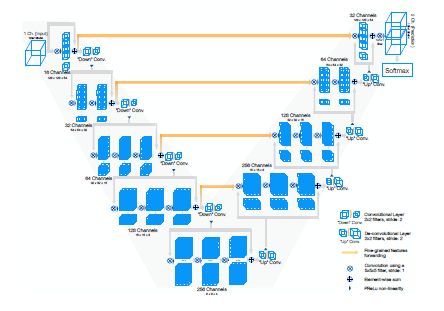
\includegraphics[width=\linewidth]{images/militari.png}
  \caption{V-Net Architecture using FCNN \cite{milletari_vnet}}
  \label{fig:miletari}
\end{figure}

Most proposed deep learning systems designed for segmenting medical images are tailored to the particular technology and anatomical modality. As an alternative to these approaches, Gibson et al \cite{gibson_niftynet:_2018} propose a general framework, termed \textit{NiftyNet}, intended to address the general medical imagery analysis task from image analysis through computer-aided intervention. This system, depicted in \ref{fig:gibson1}, uses the TensorFlow framework and is inspired by VGG. \textit{NiftyNet} is designed to provide a modular deep-learning pipeline for medical imaging applications for segmentation, regression and image generation for diagnostic analysis of medical imagery. As shown in \ref{fig:gibson1}, the NiftyNet pipeline includes data loading, data augmentation, network architectures, loss functions and evaluation metrics which are designed specifically for medical image analysis. Unique among the systems reviewed for this paper, \textit{NiftyNet} approaches an enterprise-level application for medical imagery including cross-platform support, the ability to conduct research in one part of the DL pipeline without the requirement to reproduce the other parts of the pipeline, visualization tools, built-in data augmentation and model distribution and support.  This system was tested in a variety of applications, including segmentation of spleen, kidney, gallbladder, esophagus, liver, stomach, pancreas and duodenum images. 

\begin{figure}
  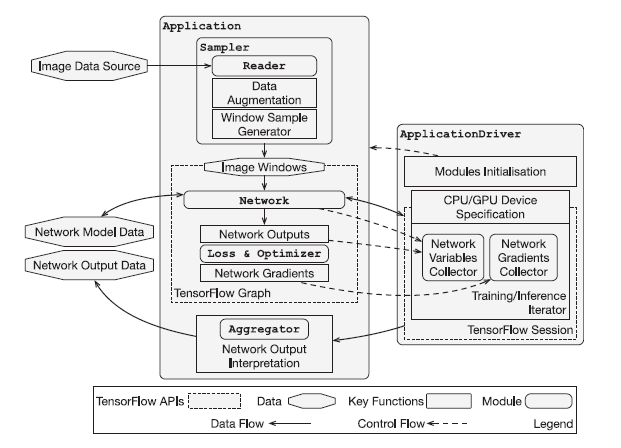
\includegraphics[width=\linewidth]{images/gibson.png}
  \caption{Architecture using FCNNs and RCF-RNNs \cite{gibson_niftynet:_2018}}
  \label{fig:gibson1}
\end{figure}

Avendi et al \cite{avendi_combined_2016}, the problem of both detecting and segmenting the cardiac left ventricle (LV) in MR images is investigated using deep learning to train a deformable model. The problem of LV detection - not germane to the topic of this survey - is implemented using CNNs. Once detected, stacked encoders are used to estimate the LV shape. Using this estimate a deformable model is used by a refines the shape of the LV for better segmentation. Used 45 LV MRI examples from the dataset from the MICCAI 2009 LV segmentation challenge and claimed better than SOTA results. Uses 6-12 MR slices of the heart. Three stages are used to estimate the LV volume and ejection fraction: a CNN is used to locate the ROI, stacked autoencoders are used to infer the LV shape and finally a deformable model is used to refine the shape. Each of the three stages is trained separately. Once the ROI is found stacked autoencoders estimate the shape of the LV. This estimate is used to initialize the deformable model. The deformable model minimizes an energy function but is prone to shrink inward due to papillary muscles but this is minimized by using the AE-inferred shape to initialize the deformable model. The minimum energy deformed shape is smoothed by comparing neighboring slices using quadratic polynomials. 

\begin{figure}
  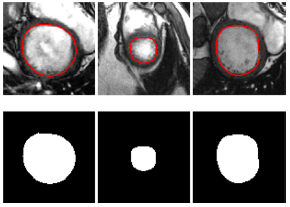
\includegraphics[width=\linewidth]{images/avendi.png}
  \caption{Manually segmented LV (top) with autoencoder generated mask (below) \cite{avendi_combined_2016}}
  \label{fig:avendi.png}
\end{figure}

In \cite{zhao_deep_2018}, Zhao et al describe an architecture that combines fully convolutional neural networks with conditional random fields (CRFs). Three networks are trained, one each for the axial, coronal and saggital views. CRFs are implemented using recurrent neural networks (CRF-RNN) and minimizes an energy function across labeled pixels in the image. Training is conducted on labeled image patches with possible labels of healthy tissue, necrosis, edema, non-enhancing core and enhancing core. The training of the networks used three steps: 1. Train the FCNNs with image patches, 2. Train the CRF-RNNs with image patches while fixing the parameters of FCNNs, 3. The entire network is trained using image slices. Images were pre-processed with N4ITK and intensity normalization. Post-processing included removal of small 3d-connected regions and using thresholding to remove false labels.

\begin{figure}
  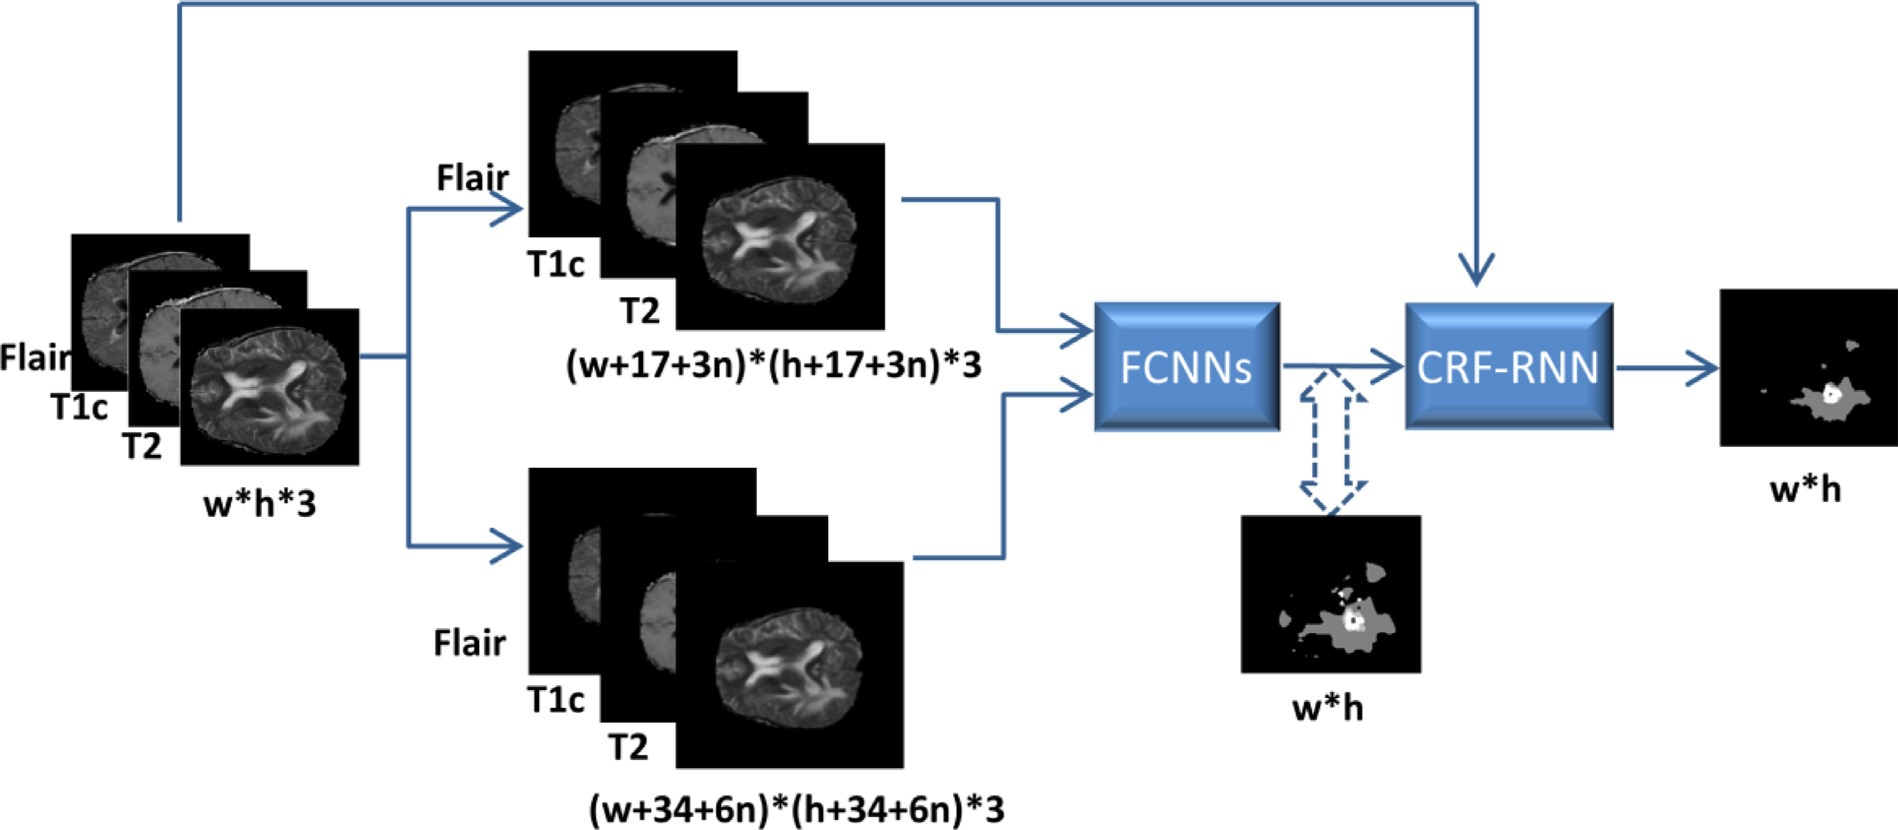
\includegraphics[width=\linewidth]{images/zhao1.jpg}
  \caption{Architecture using FCNNs and RCF-RNNs \cite{zhao_deep_2018}}
  \label{fig:zhao1}
\end{figure}

In \cite{Moeskops_automatic_segmentation}, Moeskops et al describes a segmentation system that segments a number of tissue classes using a convolutional neural network. To ensure that the method obtains accurate segmentation details as well as spatial consistency, the network uses multiple patch sizes and multiple convolution kernel sizes to acquire multi-scale information about each voxel. The method is not dependent on explicit features, but learns to recognize the information that is important for the classification based on training data. The method requires a single anatomical MR image only. The segmentation method is applied to five different data sets. Each voxel in the image is classified to one of the brain tissue classes using a CNN. Information about each voxel is provided in the form of image patches where the voxel of interest is in the centre. To allow the method to use multi-scale information about each voxel, multiple patch sizes are used. The larger scales implicitly provide spatial information, because they are large enough to recognize where in the image the voxel is located, while the smaller scales provide detailed information about the local neighbourhood of the voxel. For each of these patch sizes, different kernel sizes are trained, i.e., larger kernel sizes are used for larger patches. This multi-scale approach allows the network to incorporate local details as well as global spatial consistency. For each of the patch sizes, a separate network branch is used; only the output layer is shared. This allows the weights and biases in the CNN to be specifically optimized for each patch size and corresponding kernel size. This system was tested with data provided for the NeoBrainS12 and MRBrainS13 challenges. The largest dataset used was 15 training images and 20 test images. The smallest datasets used 5 training and 5 test images.

In \cite{NgoLC17_combining}, Ngo et al describe a methodology combining deep learning and level set methods (LSM) for the automated segmentation of the left ventricle of the heart from cardiac cine magnetic resonance (MR) data (cine MRI is a sequence of MRI frames to show movement, usually of a fluid). The authors claim that the combination of deep learning and level set (?)  is relevant for segmentation problems where the the object of interest presents large shape and appearance variations but the annotated training set is small. Specifically, level set methods are based on shape and appearance terms with small training sets. Level set methods present limitations for modelling the visual object variations. Deep learning methods can model such variations better even with relatively small amounts of annotated training but the networks often need to be regularized to generalize well. The combination of these methods brings together the advantages of both approaches, producing a methodology that needs small training sets and produces accurate segmentation results.  

Liskowski et al investigate  \cite{liskowski_segmenting_2016} segmentation of fundus (internal eye) imaging which is difficult due to variable blood vessel size, low contrast and potential presence of pathologies that differ significantly than non-diseased eye fundus images. Liskowski proposes a supervised segmentation technique that uses a deep neural network trained on a large (up to 400000) dataset. This project makes extensive use of data augmentation as the data set is derived from approximately 100 fundus images. Data augmentation using fundus image patches (cropping), geometric and color transformations (scaling, flipping, rotating and HSV adjustment) and gamma correction is used extensively. Images are preprocessed with global contrast normalization and whitening. Several architectures are used (depicted in \ref{fig:liskowski}, including a "plain" network, "no pool",  global contrast normalization and zero-phase component analysis. Further modifications are examined such as training with datasets with different weighting of fundus pathologies. This system was used with three datasets representing subjects of different ages and ethnicities, which are represent diverse fundus structure. 

\begin{figure}
  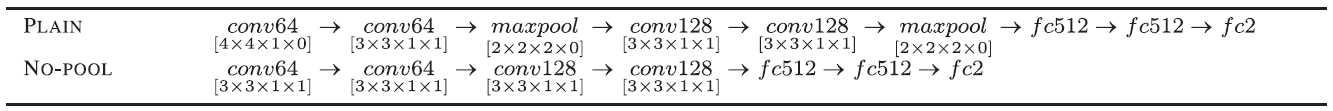
\includegraphics[width=\linewidth]{images/liskowski.png}
  \caption{Architecture for fundus imagery segmentation \cite{liskowski_segmenting_2016}}
  \label{fig:liskowski}
\end{figure}

Kamnitsas et al \cite{kamnitsas_efficient_2017} use a dual pathway, 11-layer, three dimensional CNN for brain lesion segmentation. The architecture was designed after an in-depth analysis current networks proposed for similar applications, stressing the limitations of such systems. To address the computational complexity of three dimensional processing, a dense training scheme is proposed that combines the processing of adjacent image patches into one pass while accommodating any class imbalance encountered in the data. Kamnitsas also analyzes a proposed architecture for three dimensional CNNs that would provide enhanced discrimination and better segmentation of brain lesions. To incorporate both local and larger contextual information, a dual pathway architecture that processes the input images at multiple scales is proposed. Post-processing uses a 3D fully CRF which is designed to remove false positives. 

Prasoon et al \cite{prasoon_deep_2013} propose an extension to the voxel and pixel based segmentation approach by simultaneously classifying the XY, YZ and XZ planes of a 3D volume by integrating three 2D CNNs, each having a one-to-one association with a planar slice of the three dimensional image.  This system is used to segment tibial cartilage of knee MRI scans. The system is trained on 25 annotated volumes and tested on 114 scans. The advantage to this method is that two-dimensional analysis using CNNs is comparatively well understood, avoiding some of the difficulties encountered with three dimensional CNN approaches.  

Zhang et al \cite{zhang_deep_2015} investigate segmentation of infant brain tissue images. At six to eight months of age, the brain white and gray matter exhibit virtually the same intensity on MR images, complicating the segmentation of such tissues. To address this difficulty, a deep CNN is used to segment these \textit{isointense} brain tissues. To distinguish between WM and GM tissue, multiple MR images are collected using different imaging techniques. In particular, T1, T2 and Fractional Ansiotropy (MR processing mode) images are input to CNNs in various patch sizes. This results in the detection of increasingly complex features and discrimination of brain WM, GM and cerebrospinal fluid. Information from T1, T2 (brain images), and fractional ansiotropy (FA) images as inputs were used to generate the segmentation maps as outputs. This system uses small CNNs, with 7 layers and fewer than 7M parameters. The effect of patch size on the detection of WM, GM and CSF is shown in \ref{fig:zhangbaby}.

\begin{figure}
  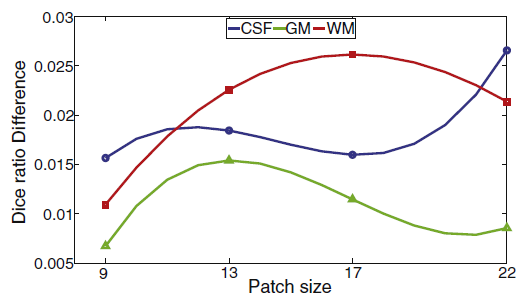
\includegraphics[width=\linewidth]{images/zhangbaby.png}
  \caption{Effect of patch size on detection of infant white matter (WM), gray matter (GM) and cerebrospinal fluid (CSF) \cite{zhang_deep_2015}}
  \label{fig:zhangbaby}
\end{figure}

\section{Weakly-Supervised Learning or Learning Transfer} 
Before discussing purely unsupervised learning, we present several weakly-supervised learning approaches. Motivated by the use and availability of datasets that are not exhaustively annotated such methods use image-level semantics to propose segmentation for an input image. An example of an image with associated semantic information is presented in \ref{fig:pathakfig}. The semantic information usually consists of tags that describe objects in the image but provide no information on the location of the objects within the image \cite{zhang2014probabilistic}. These methods use the semantic information provided to create a proposed segmentation, usually by constructing a graph that describes the proposed segmentation \cite{Pathak_2015_ICCV} \cite{zhang2014representative}. An example of an image segmented using a semi-supervised graph-based technique is presented in \ref{fig:zhanggraph}.

\begin{figure}
  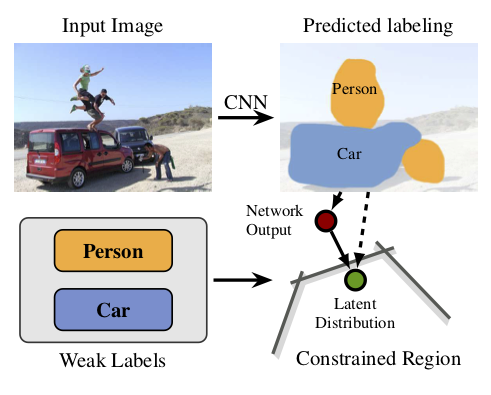
\includegraphics[width=\linewidth]{images/pathaktaggedimage.png}
  \caption{Image and tags for semi-supervised segmentation \cite{Pathak_2015_ICCV}}
  \label{fig:pathakfig}
\end{figure}

\begin{figure}
  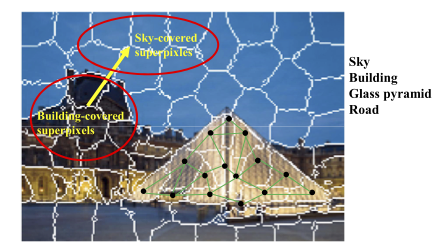
\includegraphics[width=\linewidth]{images/ZhangGraphed.png}
  \caption{Graph-based segmentation resulting from tagged semantic information \cite{zhang2014representative}}
  \label{fig:zhanggraph}
\end{figure}

Liu et al use \cite{liu2015crf} conditional random fields to propose a segmentation mask. Unlike other semi-supervised methods, this technique uses a CNN pre-trained on ImageNet to generate deep features for CRF learning. The ImageNet pre-training is transferred to the to segment images by constructing superpixels. Then the CRF parameters are learned using a structured support vector machine (SSVM). To fully exploit context information in inference, we construct spatially related co-occurrence pairwise potentials and incorporate them into the energy function. Labeling of object pairs that frequently co-occur in a certain spatial layout while avoiding implausible labelings during inference. (Weizmannhorse, Graz-02, MSRC-21, Stanford Background and PASCAL VOC 2011 datasets).

Chen et al \cite{chen_deeplab:_2018} present an application of onvolution with upsampled filters (termed ‘atrous convolution’).  Atrous convolution allows explicit control of the resolution at which feature responses are computed within DCNN. Also allows enlargement of the field of view of the filters to incorporate larger context without increasing the number of parameters or the amount of computation. Second, atrous spatial pyramid pooling (ASPP) to segment objects at multiple scales. ASPP probes an incoming convolutional feature layer with filters at multiple sampling rates and effective fields-of-views, thus capturing objects as well as image context at multiple scales. Third, localization of object boundaries by combining methods DCNN methods and probabilistic graphical models. (PASCAL VOC-2012 semantic image segmentation task, mIOU, PASCAL-Context, PASCAL-Person-Part, and Cityscapes). Code is available.

Brosch et al \cite{brosch_deep_2015}, propose a segmentation approach using deep convolutional encoder networks as applied to the segmentation of multiple sclerosis (MS) lesions in MRI. The Brosch model has convolutional and deconvolutional layers with feature extraction and segmentation prediction in a single network.  Feature learning approaches are typically patch-based but this model learns features from entire images, eliminating problems with patch selection and redundant calculations at the overlap of neighboring patches. Network also uses a novel objective function that works well for segmenting underrepresented classes (such as MS lesions but this might be more generally extendable). Varied number of training samples (5 to 250) shows that segmentation performance is greatly improved by having a representative data set.(MS Lesion Challenge 2008 dataset). 



\subsection{Sparse Training Data}

Ronneberger et al \cite{ronneberger_u-net:_2015} propose an approach for limited training data availability by relying on extensive use of data augmentation to increase the size of training datasets. The architecture consists of a contracting path to capture context and a symmetric expanding path that enables precise localization. Such a network can be trained end-to-end from very few images and outperforms the prior best method (a sliding-window CNN) for segmentation of neuronal structures in electron microscopic stacks. Using the same network trained on transmitted light microscopy images (phase contrast and DIC), won the ISBI cell tracking challenge 2015 in these categories by a large margin. Moreover, the network is fast. Segmentation of a 512x512 image takes less than a second on a recent GPU.  (ISBI dataset) [contracting path appears to mean that the image is downsampled or pooled.]

\section{Unsupervised Learning}

A study on whether Neural Networks can learn a good feature representation that captures similarities in instances - instead of classes - is introduced in \cite{Wu_2018_CVPR}. This is done by making the feature to be discriminative of individual instances. This study is powered by the fact that supervised Neural Networks have the ability to distinguish similarities among a certain category without being told to do so. Wu et al study whether this observation can be extended to the fully unsupervised domain. 

Now we will proceed to study some unsupervised techniques for some of the most influential areas of research in deep learning.

\subsection{Autonomous driving/Depth estimation/Pose estimation}

With the rise of autonomous vehicles, more and more authors are focusing on depth estimation techniques and segmentation techniques for driving footage. The need of unsupervised methods in these areas is increasing due to the variability of the data. Therefore, training an algorithm without any labels makes sense since it could provide more robustness in unexpected situations. If unsupervised learning succeeds in these areas it would be a breakthrough, since anyone could record footage from their personal phone or camera and use it to train their algorithm. In \cite{Li_2018_CVPR} and  \cite{shu_unsupervised_2016} they methods for unsupervised segmentation. In the first paper, they work with video and they propose a method that works by transferring the knowledge encapsulated in image-based instance embedding networks. They adapt the instance networks trained on static images to video object segmentation and incorporate the embeddings with objectness and optical flow features, without model retraining or online fine-tuning. The instance embedding network produces an embedding vector for each pixel that enables identifying all pixels belonging to the same object. Though trained on static images, the instance embeddings are stable over consecutive video frames, which allows us to link objects together over time. In the second paper, they work with 3D shapes and they propose an Automatic segmenting of a single 3D shape or co-segmenting a family of 3D shapes using deep learning. The algorithm consists of three stages i) decompose each 3D shape of interest into singular patches to generate over-segmentation and compute signatures as low-level features, ii) in an unsupervised manner, high-level features are learned from the low-level ones, iii) segmentation results are achieved by patch clustering in the high-level feature space. 

A big field that is deeply related to this area and can be incorporated under the same category is depth estimation. Depth estimation is another notorious field that could benefit from the success of unsupervised learning. This is one of the main reasons why many authors have tried to devise new methods to work with unsupervised data. In \cite{Zhan_2018_CVPR} Zhan et al. explore stereo sequences for learning depth and visual odometry. The use of stereo sequences enables the use of both spatial (between left-right pairs) and temporal (forward backward) photometric warp error, and constrains the scene depth and camera motion to be in a common, realworld scale. Another interesting approach for depth estimation is the one presented in \cite{Mahjourian_2018_CVPR} where they consider the inferred 3D geometry of the whole scene. Then they enforce consistency of the estimated 3D point clouds and ego-motion across consecutive frames. They solve this problem with a backpropagation algorithm for aligning 3D structures. Then they combine this novel 3D-based loss with 2D losses based on photometric quality of frame reconstructions using estimated depth and ego-motion from adjacent frames. The incorporation of validity masks helps them to avoid penalizing with no useful information. 

\begin{figure}[h!]
\centering
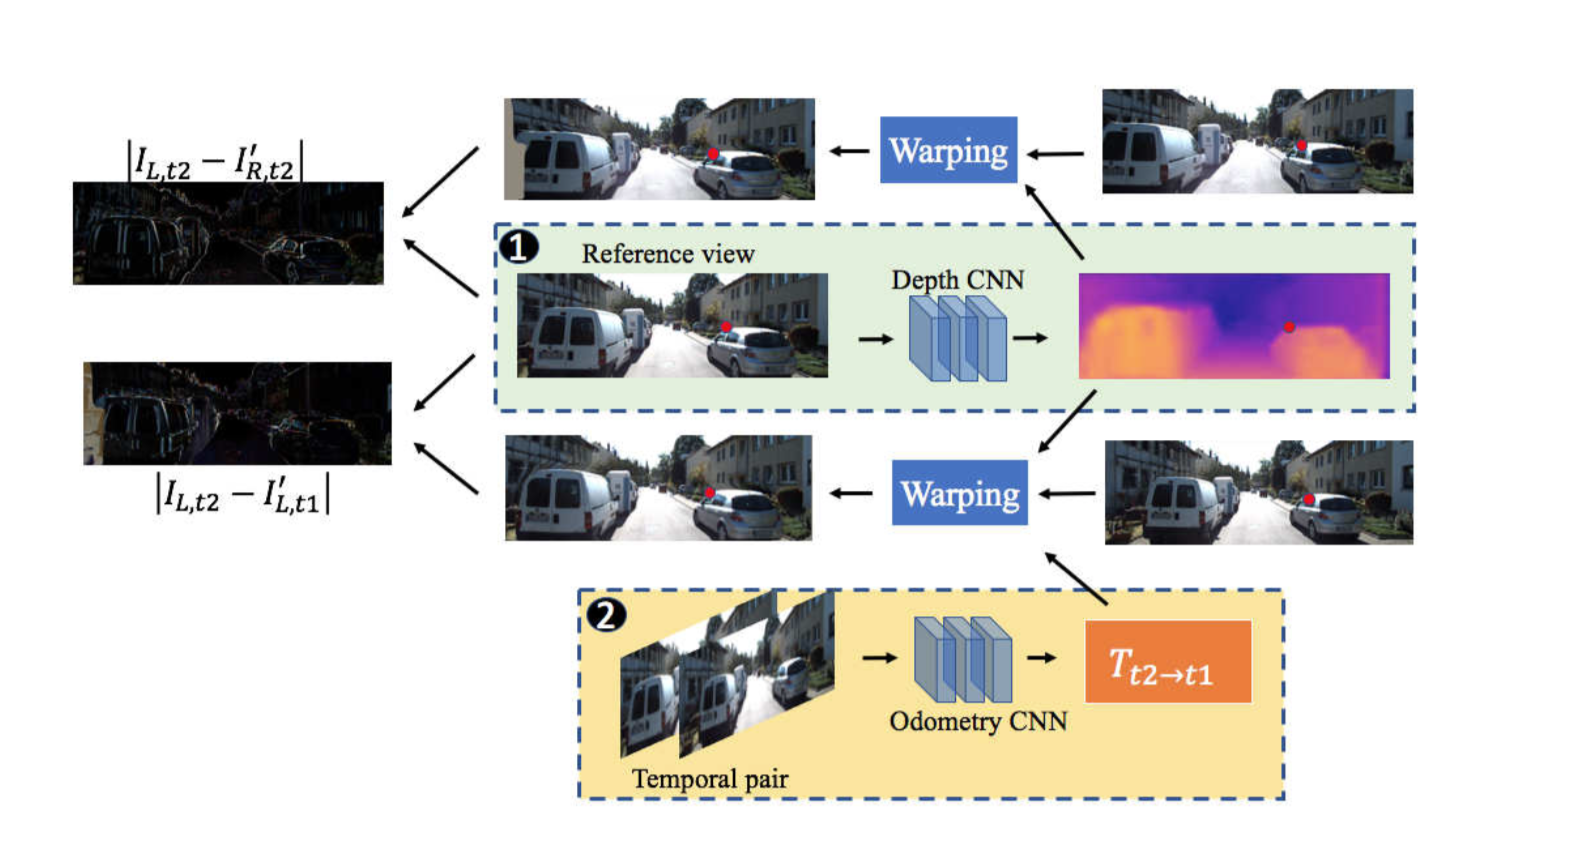
\includegraphics[width=9cm]{zhanmodel.png}
\caption{Zhan et al. model for depth estimation}
\label{fig:zhanmodel}
\end{figure}

Some approaches are focused on monocular depth, like \cite{Yin_2018_CVPR}. Yin et al. propose an unsupervised learning framework GeoNet for jointly estimating monocular depth, optical flow and camera motion from video. The foundation of our approach is built upon the nature of 3D scene geometry. An intuitive explanation is that most of the natural scenes are comprised of rigid static surfaces, i.e. roads, houses, trees, etc. Their projected 2D image motion between video frames can be fully determined by the depth structure and camera motion. Meanwhile, dynamic objects such as pedestrians and cars commonly exist in such scenes and usually possess the characteristics of large displacement and disarrangement. One of the most interesting techniques for monocular depth estimation is proposed by Kundu et al. \cite{Kundu_2018_CVPR}. They create AdaDepth, composed of  adversarial learning and explicit imposition of content consistency on the adapted target representation. 

A different approach to the ones mentioned before is the one proposed by Kanezaki et al. \cite{Kanezaki_2018_CVPR}. They use an unaligned object dataset composed of the the viewpoint labels which are treated as latent variables, and then they are learned in an unsupervised manner during the training. Their network, named RotationNet uses a partial set of multi-view images as inference. This is highly useful in real-life scenarios where there are some occluded views. Their pose alignment stategy enables them to maintain high accuracy in object categorization and pose estimation, since they have view-specific feature representations shared across classes.

\subsection{Biometrics}

Biometrics is another significant field that has many attempts at unsupervised learning. The success of unsupervised learning in biometrics would be another major breakthrough since without the need of any labels, anyone could use a dataset using free images found on the internet and using their own equipment. 

In the face recognition and landmark detection field, we found many papers that present novel and interesting approaches \cite{Dong_2018_CVPR} \cite{Genova_2018_CVPR} \cite{Wang_2018_CVPR}. In the first paper, Dong et al. present supervision-by-registration, a method for landmark detection that can be used both in video and images. Basically, it augments the training loss function with a registration loss. Therefore the detector is trained to have an ouput that is consistent with registration on unlabeled videos while being precise with the annotantions in labeled images. A differentiable Lucas-Kanade operator which performs optical flow registration while back-propagating gradients for temporal coherency, enables end-to-end training with the registration loss. In the work by Genova et al. they present a novel method in which they only use unlabeled photogrpahs. This method for is used for training a regression network from image pixels to 3D morphable model coordinates. Their method's training loss is based on features from a facial recognition network. They can be computed on-the-fly thanks to a differentiable renderer that the predicted go through.  Finally, Zhang et al.\cite{Zhang_2018_CVPR} propose an autoencoding formulation to discover landmarks as explicit structural representations.

In the field of kinematics, the work by Villegas et al. \cite{Villegas_2018_CVPR} and the work by Lv et al. \cite{Lv_2018_CVPR} are two great exponents of unsupervised learning. In the first paper, Villegas et al. propose a RNN architecture that captures the high-level properties of an input motion with a the forward kinematics layer. These properties are adapted to a target character with different skeleton bone lengths. To avoid doing the expensive procedure of collecting paired motion training sequences from different characters, their network performs a cycle consistency to solve the Inverse Kinematics problem in an unsupervised manner. In the second paper, LV et al. present an algorithm named TFusion. This algorithms is aided by the transfer learning of the pedestrians’ spatio-temporal patterns in the target domain. In a more detailed manner, the algorithm transfers the trained classifiers from the labeled origin dataset to the unlabeled target dataset. This way, the algorithm learns pedestrians’ spatial-temporal patterns. Their method also includes a learning-to-rank module as to optimize the data based on the unlabeled target data. 

\begin{figure}[h!]
\centering
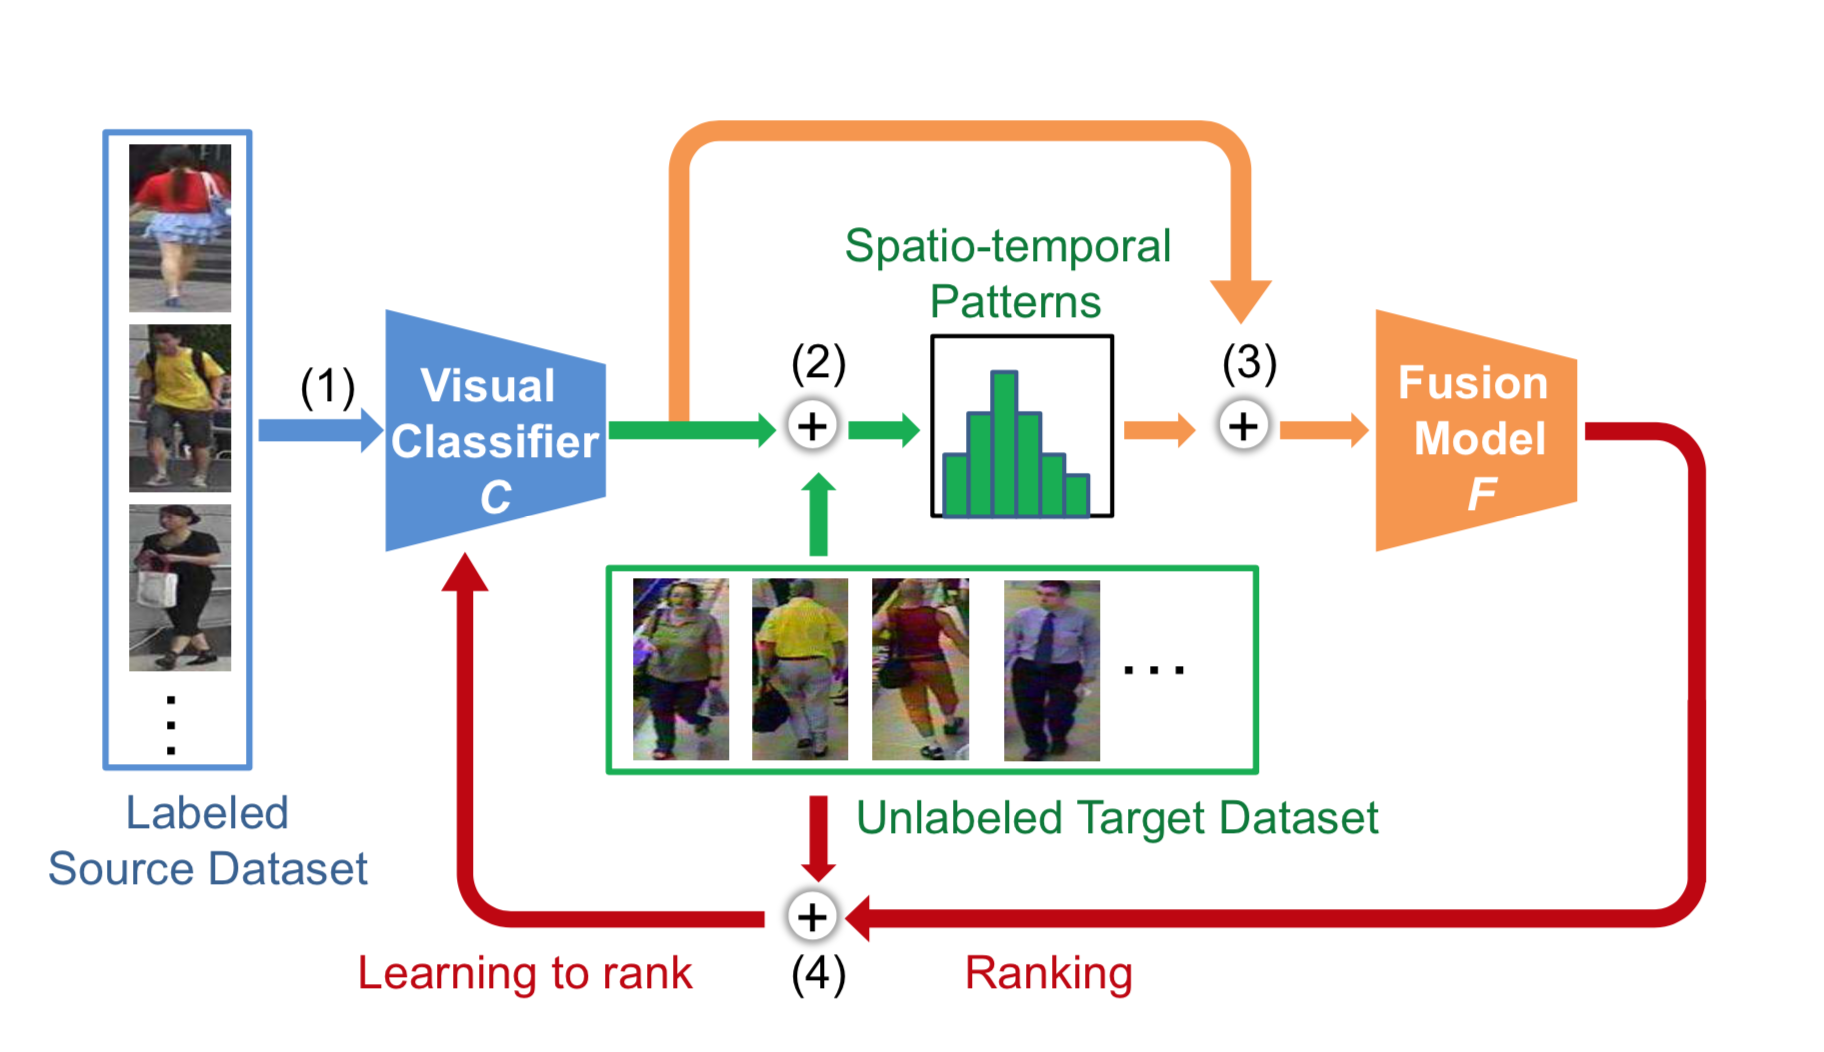
\includegraphics[width=8.5cm]{lvetal.png}
\caption{Lv et al. model for kinematics}
\label{fig:lvetal}
\end{figure}

Finally, in \cite{Wang_occlusion_2018_CVPR} they don't refer directly to face detection or biometrics, but their method is really interesting and could be applied to any of those areas. They introduce a new method which models occlusion explicitly and a new warping way that facilitates the learning of large motion. 

\subsection{Generative Adversarial Networks}

Due to the high-importance of Generative Adversarial Networks, GANs, many authors have decided to start working on unupervised approaches for these kind of networks. 
As stated in \cite{Volpi_2018_CVPR} recent work shows that a GAN can actually learn features identical to the original ones using the objective function. In their work, they further extend this idea applying two simple ideas (i) the learned feature extractor has to be domain-invariant, and (ii) using data augmentation to train the algorithm in the feature space and perform feature augmentation. This is an uncommon measure, but it is done using a feature generator.

\begin{figure}[h!]
\centering
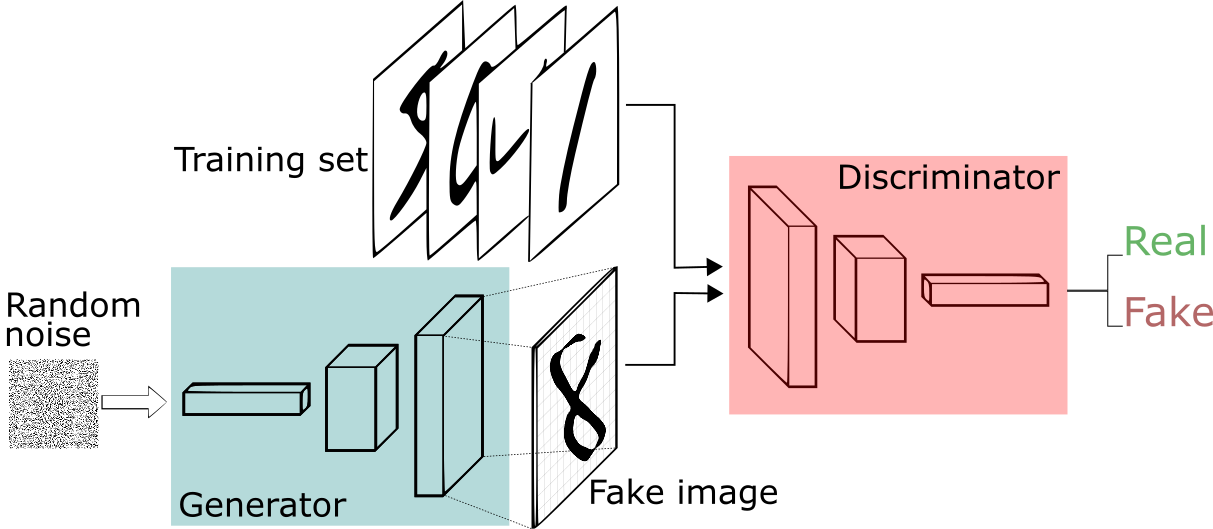
\includegraphics[width=8.5cm]{GANs.png}
\caption{Generative Adversarial Network}
\label{fig:GAN}
\end{figure}

Following this idea, authors have come up with new network structures, using GAN as their base model and adding small tweaks to combine them with unsupervised learning \cite{Hu_2018_CVPR} \cite{Dizaji_2018_CVPR} \cite{Chen_2018_CVPR} \cite{Zhang_collaborative_2018_CVPR}. All these methods share the common idea of using the GAN as the base architecture. So all of them share the same three parts that compose a GAN. A generator, a discriminator and an encoder. Some of the tweaks done to this base network include the many diverse ideas. For example, using duplex adversarial discriminators together with a GAN, create a DupGAN. This is done to achieve domain transformation and domain-invariant representation. This network consists of three parts. First of all, an encoder that works with embedded samples a generator and two discriminators. The encoder embeds samples from both domains into the latent representation. Then a generator decodes the latent representation to both source and target domains respectively conditioned on a domain code. This is followed by a generator that is pitted against one discriminator for source domain and another discriminator for target, creating a duplex discriminator. Another interesting method is created by combining a hashing function and a GAN. The resulting method is called HashGAN. It efficiently obtains binary representation of input images using an unsupervised deep learning method. HashGAN consists of three networks that compose a GAN and then they share the parameters of the encoder and discriminator. This allows the network to benefit from the adversarial loss as a data-dependent regularization in training the deep hash function. To obtain uniform frequency, minimum entropy, and consistent and independent hash bits, a novel hashing loss function is introduced for the real images. In the end, a collaborative loss in training enforces similar random inputs and hash bits for synthesized images. An approach named Re-weighted Adversarial Adaptation Network (RAAN) is created to reduce the feature distribution divergence. This will help  to adapt the classifier when the algorithm encounters disparate domain discrepancies. The authors choose to minimize the optimal transport based Earth Mover distance and reformulate it to a minimax objective function. This is done to alleviate the need of common supports in matching the feature distribution. Therefore, with this structure, the RAAN model can be trained in an adversarial manner. A similar approach is presented in Collaborative and Adversarial Network (CAN) through domain-collaborative and domain adversarial training of neural networks. CNN feature extraction blocks are combined with domain classifiers. A loos function is defined based on the hidden presentation and the domain labels. Each domain classifier is connected to the hidden representation from one block. Then all the losses from all blocks are integrated, creating a new loss function. This loss function, combined with adversarial learning is helpful to learn domain informative representations from lower blocks through collaborative learning and learn domain uninformative representations from higher blocks. Finally in the work by Pumarola et al. \cite{Pumarola_2018_CVPR} they present a novel approach for synthesizing photorealistic images of people in arbitrary poses using generative adversarial learning. They are able to perform unsupervised learning by splitting the problem into two subtasks. The first subtask consists on considering a pose conditioned bidirectional generator. It maps back the initially rendered image to the original pose. Therefore it becomes comparable to the input image without needing any training image. The second subtask, consists of a loss function that incorporates content and style terms. It aims at producing images of high perceptual quality.

\begin{figure}[h!]
\centering
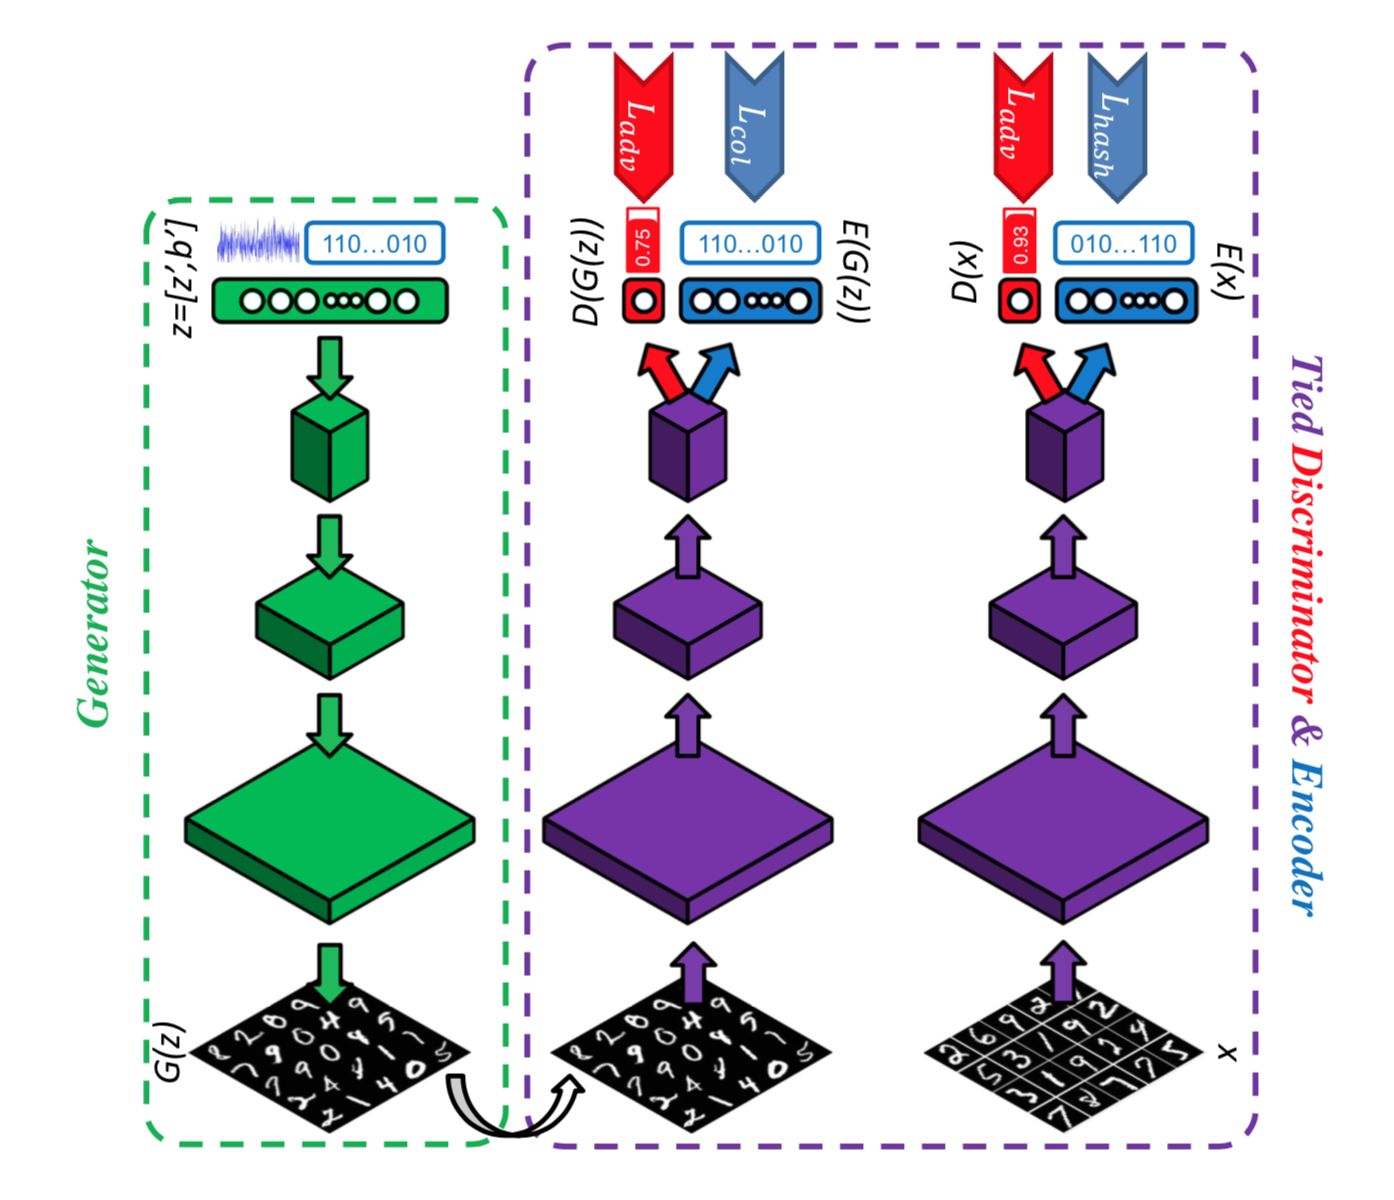
\includegraphics[width=8.5cm]{hashgan.png}
\caption{HashGAN model presented by Dizaji et al.}
\label{fig:hashgan}
\end{figure}


Before concluding this section, we would like to reference the work done in \cite{Xu_2018_CVPR} by Xu et al. They don't use a GAN architecture, but they do use muilti-way adversarial learning. They do this to minimize the discrepancy between the target and the source domain. The network that they propose is called a deep cocktail network (DCTN) and it is used to battle the domain and category shifts among multiple sources.

\subsection{Miscellaneous}

Unsupervised learning has been also applied to other areas like Current Correlation Analysis \cite{Hoshen_2018_CVPR}, saliency detection \cite{Zhang_deep_2018_CVPR}, textual grounding \cite{Yeh_2018_CVPR}, hyperspectral image \cite{Qu_2018_CVPR} and image classification  \cite{Pinheiro_2018_CVPR}. One notable example is the work by Hoshen et al. \cite{Hoshen_2018_CVPR} where they introduce a novel method named Unsupervised Correlation Analysis (UCA). This model doesn't require any correspondances between the different domains. This poses a huge advantage in front of CCA, where the models need annotations. Thanks to the unsupervised nature of the model, they can achieve multiple solutions with similar scores. They introduce a consensus-based algorithm to recover the desired solution. As for unsupervised saliency detection, Zhang et al. \cite{Zhang_deep_2018_CVPR} present a method that learns from multiple noisy labeling generated by weak and noisy unsupervised saliency methods. Their framework consists of a latent saliency prediction module and a noise modeling module that work collaboratively and are optimized jointly. For iamge classification, Pinheiro et al. \cite{Pinheiro_2018_CVPR} proposed a method based on similarity learning. Classification is performed by computing similarity between model representations of each category. They use a pairwise similarity function to perform this. Finally, images from the target domain are compared to the prototypes. The one that has a best match with the image is outputed.


\begin{figure}[h!]
\centering
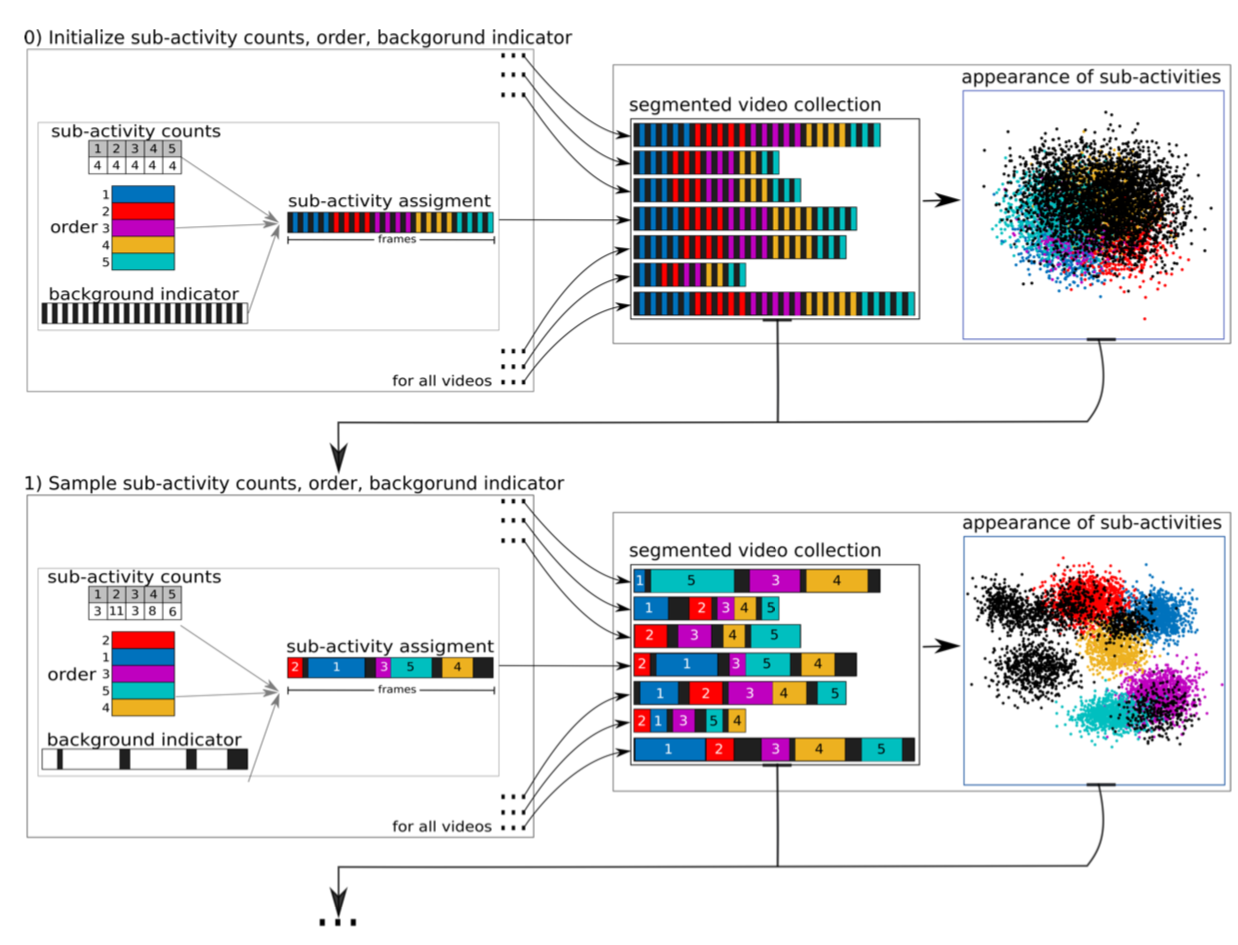
\includegraphics[width=8.5cm]{Subactivity.png}
\caption{Sener et al. model for video segmentation}
\label{fig:Subactivity}
\end{figure}

One really interesting method that could easily be applied to medical segmentation is proposed in \cite{Sener_2018_CVPR} by Sener et al. Their method, presented in Figure \ref{fig:Subactivity}, performs segmentation of complex activities from video into multiple steps, or sub-activities in an unsupervised manner. They achieve this by using and iterative discriminative-generative approach. This approach discriminatively learns sub-activities from the visual features included in the videos and then generates models of the temporal structure of these sub-activities. To avoid any misclassification issues, they account frames unrelated to the activities using a background model. 


In \cite{romero_unsupervised_2016} describes single-layer and deep convolutional networks for remote sensing data analysis. Direct application to multi- and hyperspectral imagery [is this close enough to medical? not sure] of supervised convolutional networks difficult due to high input data dimensionality and the  small amount of labeled training data. Uses greedy layerwise unsupervised pretraining coupled with a highly efficient algorithm for unsupervised learning of sparse features. Sparse representations and enforces both population and lifetime sparsity of the extracted features. Algorithm is sufficiently expressive extracted for: classification of aerial scenes and land-use classification from multi- and hyperspectral images. Better than standard principal component analysis (PCA) and kernel PCA. Results show that single-layer convolutional networks can extract powerful discriminative features only when the receptive field accounts for neighboring pixels and are preferred when the classification requires high resolution and detailed results while deep architectures outperform single-layer variants by capturing increasing levels of abstraction and complexity features.

In \cite{affonso_deep_2017} [Probably not worth keeping but here's another paper] This paper investigates the classification of the quality of wood boards based on their images. For such, it compares the use of deep learning, particularly CNNs, with the combination of texture-based feature extraction techniques and traditional techniques: Decision tree induction algorithms, Neural Networks, Nearest neighbors and Support vector machines. Finally are pointed out some perspectives of futures developments with the application of Active learning and Semi supervised methods.

In \cite{cimpoi_deep_2015}, Uses texture to aid segmentation. The texture descriptor, FV-CNN, is obtained by Fisher Vector pooling of a CNN filter bank. FV-CNN can incorporate multiscale information and describe regions of arbitrary shapes and sizes. Our approach is particularly suited at localizing “stuff” categorites as well as general open set performance. (Flickr, MIT indoor scenes, MSRC, OpenSurfaces)

In \cite{hoo-chang}  Three major techniques that successfully employ CNNs to medical image classification: training the CNN from scratch, using off-the-shelf pre-trained CNN features, and conducting unsupervised CNN pre-training with supervised fine-tuning. Another effective method is transfer learning. Understudied factors of employing deep convolutional neural networks to computer-aided detection problems: different CNN architectures, the influence of dataset scale and spatial image context on performance, and transfer learning from pre-trained ImageNet can be useful. Two specific computer-aided detection (CADe) problems, thoraco-abdominal lymph node detection and interstitial lung disease (ILD).



In \cite{brosch_deep_2016}, a segmentation approach based on deep 3D convolutional encoder networks with shortcut connections. Applied to multiple sclerosis (MS) lesion segmentation in MRIs. CNN with two interconnected pathways, a convolutional pathway, which learns increasingly more abstract and higher-level image features, and a deconvolutional pathway, which predicts the final segmentation at the voxel level. Joint training of the feature extraction and prediction pathways allows for automatic learning of features at different scales that are optimized for accuracy for any given combination of image types and segmentation task. MOST SIGNIFICANT (?): shortcut connections between the two pathways allow high- and low-level features to be integrated, which enables the segmentation of lesions across a wide range of sizes. (MICCAI 2008 and ISBI 2015 challenges)

In \cite{brosch_deep_2015} similar to above but with more data/testing.  (MICCAI
2008 and ISBI 2015 challenges) 

\section{USE OF UNSUPERVISED LEARNING IN MEDICAL IMAGING}

\begin{figure*}[h!]
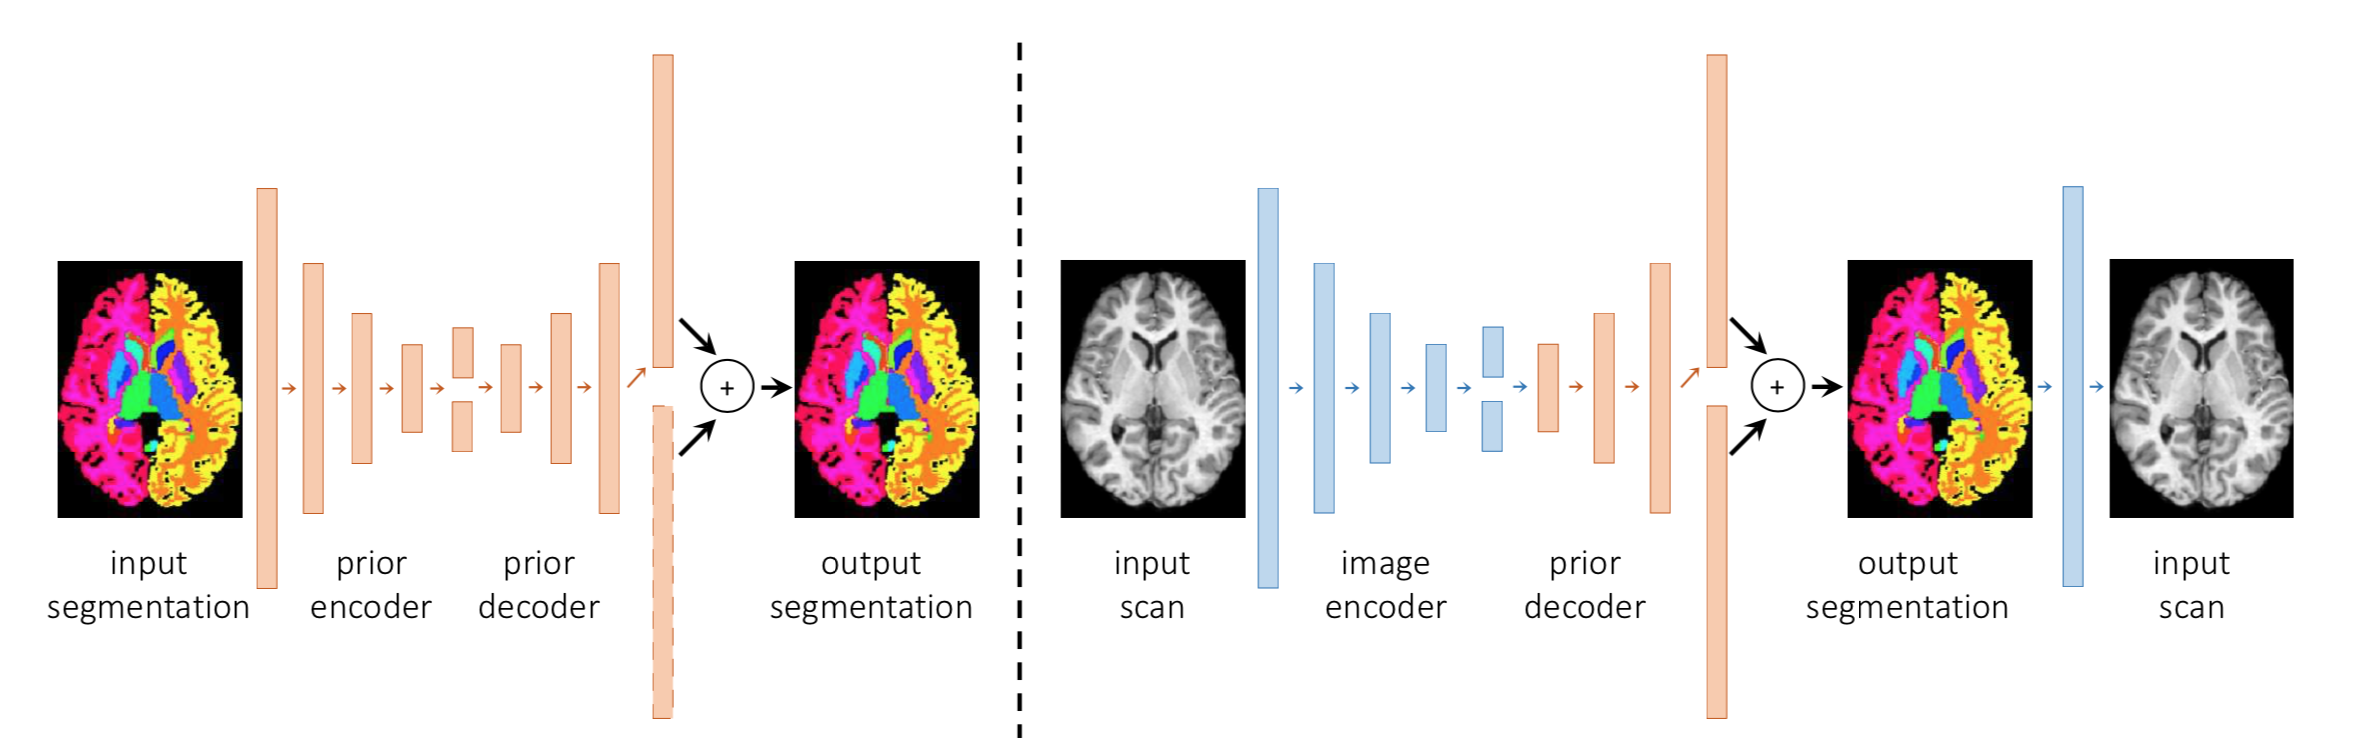
\includegraphics[width=\textwidth,height=5cm]{dalca.png}
\caption{Dalca et al. model for medical segmentation}
\label{fig:dalca}
\end{figure*}

Until July 2018, there have not been many authors that have used unsupervised learning in medical imaging. Two really interesting approaches were introduced at the Computer Vision and Pattern Recognition Conference from 2018 in Salt Lake City, Utah. The first work, presented by \cite{Balakrishnan_2018_CVPR} is focused on a fast learning-based algorithm for deformable, pairwise 3D medical image registration. Due to the need to optimize an objective function independently for every image, registration methods are really time consuming, specially when working with large amounts of data. They use a parametric function to define registration, and they optimize the parameters using the desired set of images. If the system registers a new image, they compute a registration field using the learned parameters. The function is modedeled using a CNN and then impose smoothness constraints on the registration range while using a layer containing a spatial transform to reconstruct one image from another. Their method doesn't require any supervised information. In the second work, Dalca et al. \cite{Dalca_2018_CVPR} use unpaired segmentation images which are used to build an anatomical prior. The segmentations can be originated from a different dataset, including imaging modality, than the one that is being employed for the actual task. Their model, which can be seen in Figure \ref{fig:dalca} contains a probabilistic model where a CNN employs the things that have been learned prior. They study their model using MRI images to prove that anatomical prior actually enables unsupervised segmentation. This is quite novel since usually standard convolutional networks require annotated data. These model can be applied to a wide range of novel clinical problems where there is non or almost none annotated data.



\addtolength{\textheight}{-12cm}   % This command serves to balance the column lengths
                                  % on the last page of the document manually. It shortens
                                  % the textheight of the last page by a suitable amount.
                                  % This command does not take effect until the next page
                                  % so it should come on the page before the last. Make
                                  % sure that you do not shorten the textheight too much.

%%%%%%%%%%%%%%%%%%%%%%%%%%%%%%%%%%%%%%%%%%%%%%%%%%%%%%%%%%%%%%%%%%%%%%%%%%%%%%%%



%%%%%%%%%%%%%%%%%%%%%%%%%%%%%%%%%%%%%%%%%%%%%%%%%%%%%%%%%%%%%%%%%%%%%%%%%%%%%%%%


\section{CONCLUSIONS}
In this paper we have reviewed some of the most common supervised methods for medical segmentation. We have also reviewed some of the most notorious unsupervised learning methods for some of the major areas in Computer Vision. For now, results-wise, unsupervised learning isn't always an improvement over supervised learning. Since it hasn't been widely applied to medical segmentation we intend to explain and highlight some of the most innovative unsupervised learning methods so that they can be used in medical applications. 

\bibliographystyle{ieeetr}
\bibliography{CS6000Survey}
%\nocite{*}

\end{document}
